% HFUT_Courge_Project
\documentclass[UTF8]{ctexart}
% \usepackage{fancyhdr}
\usepackage{graphicx}
% \usepackage{titlesec}
% \usepackage{titletoc}
\usepackage{listings}
\usepackage{appendix}
\usepackage{bm, amsmath,amsfonts}
\usepackage{multirow}
\usepackage[a4paper,left=3.4cm,right=3cm,top=2.5cm,bottom=2.54cm]{geometry}
% \renewcommand{\contentsname}{\zihao{3} 目\quad 录}
% \renewcommand{\abstractname}{\zihao{3} 摘\quad 要}
%页眉页脚设置
% \pagestyle{fancy}
\pagestyle {plain}
% \fancyhf{}
% \cfoot{\thepage}
% \rhead{\kaishu~XX课程设计~}

%目录页设置
% \titlecontents{section}[0em]{\zihao{4}\bf }{\thecontentslabel\ }{}
% {\hspace{.5em}\titlerule*[4pt]{$\cdot$}\contentspage}
% \titlecontents{subsection}[2em]{\vspace{0.1\baselineskip}\zihao{-4}}{\thecontentslabel\ }{}
% {\hspace{.5em}\titlerule*[4pt]{$\cdot$}\contentspage}
% \titlecontents{subsubsection}[4em]{\vspace{0.1\baselineskip}\zihao{-4}}{\thecontentslabel\ }{}
% {\hspace{.5em}\titlerule*[4pt]{$\cdot$}\contentspage}
%代码设置
\RequirePackage{listings}
\RequirePackage{xcolor}
\definecolor{dkgreen}{rgb}{0,0.6,0}
\definecolor{gray}{rgb}{0.5,0.5,0.5}
\definecolor{mauve}{rgb}{0.58,0,0.82}
\lstset{
	numbers=left,  
	frame=tb,
	aboveskip=3mm,
	belowskip=3mm,
	showstringspaces=false,
	columns=flexible,
	framerule=1pt,
	rulecolor=\color{gray!35},
	backgroundcolor=\color{gray!5},
	basicstyle={\ttfamily},
	numberstyle=\tiny\color{gray},
	keywordstyle=\color{blue},
	commentstyle=\color{dkgreen},
	stringstyle=\color{mauve},
	breaklines=true,
	breakatwhitespace=true,
	tabsize=3,
}
%------------------------------------------------------------------------
%正文部分
\begin{document}
 \begin{abstract}
 	% \pagestyle{plain}
 	% \thispagestyle{empty}
 	% \zihao{-4}
BP神经网络是一种具有反向修正功能的神经系统,具有的非线性特性和学习能力且已被证明具有逼近任意有界函数的能力。它有能力辨识那些不能线性化的非线性系统,不需要预先知道被测系统的模型。BP神经网络结构具有较强的自适应能力,并行处理和高度鲁棒性,采用神经网络方法设计的控制系统将具有更强的实时性,更强的适应能力和更强的鲁棒性。针对BP神经网络收敛速度慢等缺点,本文对带随机噪声的二阶系统的差分结构进行了改进BP神经网络的辨识模拟。
	% \\[0.5cm]
	
	\textbf{关键字}:\quad BP神经网络 \quad 改进BP神经网络 \quad 仿真 \quad 系统辨识

	% \newpage
\end{abstract}

\renewcommand\abstractname{Abstract}
\begin{abstract}
The BP neural network is a neural system with inverse correction function, which has nonlinear characteristics and learning ability and has been proven to have the ability to approximate arbitrary bounded functions. It has the ability to identify nonlinear systems that cannot be linearized without the need to know the model of the system under test in advance. The BP neural network structure has strong adaptive ability, parallel processing and high robustness. The control system designed by neural network method will have stronger real-time performance, stronger adaptability and stronger robustness. Aiming at the shortcomings of BP neural network, such as slow convergence speed, this paper improves the BP neural network identification of the difference structure of the second-order system with random noise.

\textbf{Keywords}:\quad BP neural network \quad Improved BP neural network \quad Simulation \quad System Identification
\end{abstract}

% \tableofcontents\thispagestyle{empty}
% \newpage
% \setcounter{page}{1}
\section{引言}
传统的系统辨识方法有着很多的不足,主要表现在:它要求研究人员给出系统模型的结构及阶次,即模型的建立要立足于函数的求解,这个过程是很难实现,因此确定模型参数的系统辨识理论的研究和应用都还局限于线性系统。人工神经网络是由大量而简单的神经元按某种方式连接形成的智能仿生动态网络,依靠计算机强大处理能力来实现对信息的处理。其具有的非线性特性和学习能力,为解决复杂的非线性、不确定系统的辨识问题,开辟了一条有效的途径。它不需要预先知道被测系统的模型就可以将系统模型辨识出来,这是神经网络辨识的优势所在。

人工神经网络是近年来的热点研究领域,涉及到电子科学与技术、信息与通信工程、计算机科学与技术、控制科学与技术等很多学科,其应用领域包括:建模、时间序列分析、模式识别和控制等,并在不断的拓展。神经网络的学习算法一直是人工神经网络理论研究和应用领域中一个重要的研究领域。神经网络的学习算法一直是人工神经网络理论研究和应用领域中的一个重要研究内容,尤其是对前馈神经网络学习算法的研究,至今没有一个十分理想的解决办法。其中BP神经网络在前馈神经网络学习算法中有着最广、最具有代表性。通过对BP神经网络算法较为深入的研究,提出了改进算法。
\section{系统辨识}

系统辨识是根据系统的输入输出时间函数来确定描述系统行为的数学模型。现代控制理论中的一个分支。通过辨识建立数学模型的目的是估计表征系统行为的重要参数,建立一个能模仿真实系统行为的模型,用当前可测量的系统的输入和输出预测系统输出的未来演变,以及设计控制器。对系统进行分析的主要问题是根据输入时间函数和系统的特性来确定输出信号。对系统进行控制的主要问题是根据系统的特性设计控制输入,使输出满足预先规定的要求。系统辨识是在已知或测得系统输入和输出数据的基础上,从一组给定的模型类中,确定一个与所测系统等价的模型。系统辨识要素为:数据:指系统过程的输入数据和输出数据,它是辨识的基础。模型类:指各种已知的系统过程模型集合,它是辨识时寻找模型的范围。系统辨识的等价准则:指系统行为相似性、系统效用等同性的识别标准,它是辨识优化的目标。辨识的实质就是按某种准则,从一组已知模型类中选择一个模型,使之能最好地拟合实际过程的动态特性。观测数据含有噪声,因此辨识建模实际上是一种实验统计的方法,所获得的模型只是与实际过程的外特性等价的一种近似描述。

所谓辨识建模是从实验数据出发,根据辨识的目的以及对过程已有的验前知识,预先给出一个模型类(线性的、非线性的、定常的、时变的、连续的、离散的…)进行拟合。无论是基于算法的辨识还是基于神经网络的辨识方法,都应当考虑模型、输入信号、以及误差准则的选择这三个基本问题:
\subsection{模型的选择}
模型是在某种意义下对于实际系统的一种近似描述,正确选择模型依赖于模型的用途和兼顾其精确性和复杂性问题。如果所建立的模型是用于系统分析的,则所需的模型必须把精确性放在首位,此时模型可能变得比较复杂。若建立的模型主要用于实时控制,可忽略次要因素,只考虑其主要因素,使模型简单些。在建立实际系统模型时,由于存在精确性和复杂性的矛盾,则要找到解决矛盾的折衷方法。反映在选择多层网络模型上,由于隐层及其节点数的确定目前还没有理论上的明确指导,折衷的方法即体现在通过多次仿真实验,找出能在给定准则下逼近原系统的最简单的多层网络模型。
\subsection{输入信号的选择}
为了能够辨识实际系统,输入信号必须满足一定条件。第一,在辨识时间内,输入信号必须是持续激励的,即输入信号必须充分激励系统的所有模态,使系统所有的模态都在模型中得以体现。从频谱观点看,输入信号的频谱必须足以覆盖系统的频谱。第二,输入信号的最优设计问题,即设计输入信号使给定问题的辨识精度最高。反映在BP网上,训练样本的选择应能使训练好的网络对所有模式类的输出响应都比较接近于实际输出。常用的输入信号有白噪声或伪随机信号。
\subsection{误差准则的选择}
误差准则是用来衡量模型接近实际系统的标准,它通常表示为一个误差的泛函,记作$ J(\theta)=\sum^l_{i=1}f[e(k)] $式中,$ f(\cdot) $是$ e(k) $的函数,用得最多的是平方函数,即$ f[e(k)]=e^2(k) $
\section{BP神经网络}
BP网络是一种利用误差反向传播训练算法的神经网络,简称BP(Back Propogation)网络,结构图如图1所示,是一种有隐含层的多层前馈网络,系统地解决了多层网络中隐含单元连接权的学习问题。 如果网络的输入节点数为M、输出节点数为L,则此神经网络可看成是从M维欧氏空间到L维欧氏空间的映射。这种映射是高度非线性的。
\begin{figure}[htbp]
	\centering
	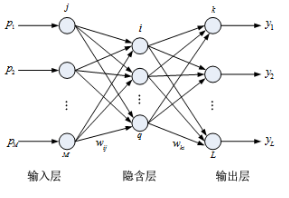
\includegraphics [width=0.3\textwidth]{fig/png1.png}
	\caption{BP神经网络结构图}
	\label{fig:my_png_1}
\end{figure}
\subsection{BP算法原理}
 BP学习算法的基本原理是梯度最速下降法,它的中心思想是调整权值使网络总误差最小。也就是采用梯度搜索技术,以期使网络的实际输出值与期望输出值的误差均方值为最小。网络学习过程是一种误差边向后传播边修正权系数的过程。这种学习的过程就是训练的过程,是神经网络各神经元连接方式、权值和阈值的调整过程,更是辨识的过程。学习的方法是使所确定的误差函数达到最小值,从而得到隐含在被测系统的输入输出数据之间的关系。

BP网络的每一层连接权值都可通过学习来调节。多层网络运行BP学习算法时,实际上包含了正向和反向传播两个阶段。在正向传播过程中,输入信息从输入层经隐含层逐层处理,并传向输出层,每一层神经元的状态只影响下一层神经元的状态。如果在输出层不能得到期望输出,则转入反向传播,将误差信号沿原来的连接通道返回,通过修改各层神经元的权值,使误差信号最小。

(1)信息的正向传递:
隐含层中第j个神经元的输出为
$$ y_{j}(n)=\varphi_j(\sum^{p}_{i=0}w_{ji}(n)y_i(n)) $$

对应于隐含层的函数$ \varphi_j(\cdot) $常常是S型激活函数
$$ y=\frac{1}{1-e^{-x}} $$

输出层第j个神经元的输出为
$$ y_j(n)=\psi_j(\sum^{p}_{i=0}w_{ji}(n)y_i(n)) $$

对应于输出层的函数$ \psi_j(\cdot) $常常是线性的激活函数。这是因为s型函数具有非线性放大系数功能,它可以把输入从负无穷大到正无穷大的信号,变换成-1到1之间输出,对较大的输入信号,放大系数较小;而对较小的输入信号,放大系数则较大,故可采用s型激活函数去处理和逼近非线性的输入、输出关系。不过,如果在输出层采用s型函数,输出则被限制到一个很小的范围了,若采用线性激活函数,则可使得网络输出任何值。所以只有希望对网络输出进行限制,才在输出层包含s型激活函数,而在一般情况下,均是在隐层采用s型激活函数,而在输出层采用线性激活函数。

第n个样本时,对应于第j个输出层神经元的误差信号是:
$$ e_j(n)=d_{j}(n)-y_j(n) $$

第n个样本时ide平方误差是:
$$ \xi(n)=\frac{1}{2}\sum^{p}_{j=0}e^{2}_{j}(n)  $$

平方误差的均值:
$$ \xi_{av}=\frac{1}{N}\sum^{N}_{n=1}\xi(n) $$

最终目的是让$ \xi_{av} $趋向最小。

(2)反向误差传播:
输出层的权值变化的公式如下:
$$ dw_{ji}(n)=-\eta\frac{\partial\xi(n)}{\partial w_{ji}(n)}=-\eta\cdot\delta_j(n)\cdot y_i(n) $$
其中:
$$ \delta_j(n)=(d_j(n)-y_j(n))\cdot \varphi_j(v_j(n)) $$
$$ v_j(n)=\sum^{p}_{i=0}w_{ji}(n)\cdot y_j(n) $$
隐含层的权值变化公式和输出层的类似,所不同的是,在这里:
$$ \delta_j(n)=\varphi_j(v_j(n))\cdot \sum_k(\delta_k(n)\cdot w_{kj}(n)) $$
其中,k表示的都是误差传播途径上的上一层神经元的量。

\subsection{改进的BP网络训练算法}
传统的BP算法存在以下的限制,由于实际问题很多是非线性的,局部最优的问题仍然存在,同时该算法的收敛速度慢。中间层的神经元的选择数目基本上都没有明确的理论依据,通常都是根据日常实验的经验。还有就是在对新样本就行学习操作的时候,算法就会很快忘掉过去使用的样本,同时每一个样本的特点被要求是相同的类似的才能够进行统一的处理。虽然BP网络有其重要地的意义,但在实际应用中存在不少问题:

(1)学习算法的收敛速度很慢。因为BP算法是以梯度下降法为基础的,只具有线性收敛速度,虽通过引入“势态项”增加了一定程度的二阶信息,但对算法的性质并无根本的改变。

(2)学习因子和记忆因子    没有一种选择的规则,若选的过大会使训练的过程引起振荡,若选的过小会使训练的过程更加缓慢。

(3)网络对初始值的敏感性。同一BP网络不同的初值会使网络的收敛速度差异很大。若初值权值离极小点很近,则收敛速度较快,若初值权值远离极小点,则收敛速度极慢。另外,若输入初值不合适,训练起始段就会出现振荡。

(4)网络的隐层节点个数的选择尚无理论指导,而是根据经验选取。

(5)从数学上看BP算法是一个非线性的优化问题,这就不可避免地存在局部极小问题。

针对加快收敛速度这个策略,有以下集中算法:

\begin{itemize}
\item 改变学习速度$\eta$
\item 动量法:依据误差估计把上次的调整权值计入到当前的权值调整计算中去
\item 寻找合适的传递函数
\item 降低网络灵敏度
\end{itemize}

其中,本文采取的是第3中方法,寻找合适的传递函数,加快收敛速度。在选择传输函数的时候,需要考虑到取值范围的变化,导数的变化范围。本文中函数的敏感范围是坐标原点附近的坐标。我们同事希望传递函数导数的曲线尽可能高,同时峰值区间尽可能广。标准的BP问题的输出范围是0到1,函数的导数是$ f(x)=f(x)(1-f(x)) $,变化范围是0到0.25。标准的S型函数的收敛速度很慢。为了加快收敛速度,选取函数的倒数峰值尽可能大,变化范围大,比如:
$$ f(x)=\frac{1}{1+(x^{-1}-1)^2},0<x<1 $$

通过对该函数进行单调性分析,我们可以看出该函数是单极的,独立变量的值是有界的。因此,我们引入了 扩大了独立变量的范围。得到如下的公式:
$$ f(x)=\frac{2\lambda x}{1+\lambda^2x^2} $$

对函数求一次和两次导数,得到:
$$ f^{'}(x)=\frac{2\lambda(1-\lambda^2x^2)}{(1+\lambda^2x^2)^2} $$
$$ f^{''}(x)=\frac{4\lambda^3x(\lambda^2x^2-3)}{(1+\lambda^2x^2)^3} $$
\section{改进BP神经网络的仿真}

对具有随机噪声的二阶系统的模型辨识,进行标幺化以后系统的参考模型差分方程为:
$$ z(k)=a_1z(k-1)+a_2z(k-2)+b_1u(k-1)+b_2u(k-2)+\xi(k) $$

式中,$ a_1=1.5,a_2=-0.7,b_1=1,b_2=0.5 $,$\xi$为随机噪声。由于神经网络的输出最大为1,所以,被辨识的系统应先标幺化
神经网络选用4-10-10-1型,即输入层i,隐层j包括2级,输出层k的节点个数分别为4、10、10、1个;采用Python编程实现改进神经网络的建模以及仿真。


\begin{figure}[h]
	\centering
	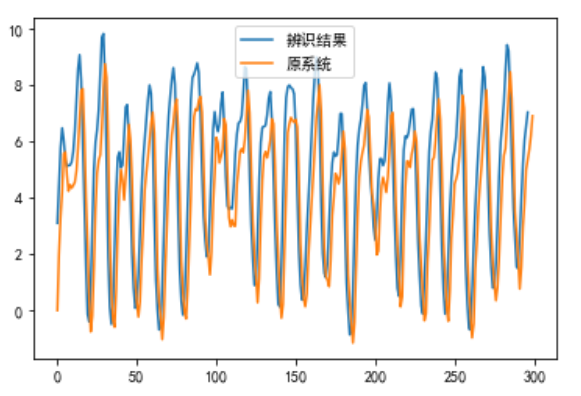
\includegraphics [width=0.6\textwidth]{fig/png_m.png}
	\caption{辨识结果}
	\label{fig:my_png_2}
\end{figure}

\begin{figure}[h]
	\centering
	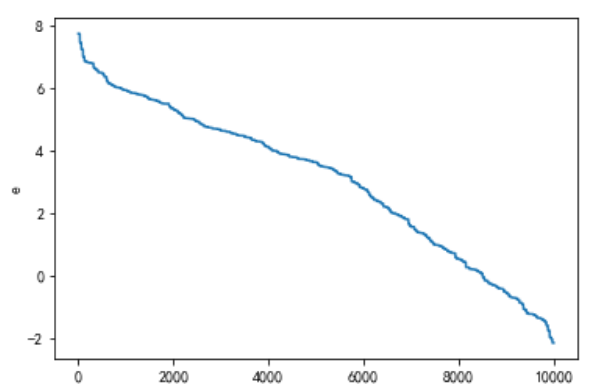
\includegraphics [width=0.6\textwidth]{fig/png_e.png}
	\caption{训练1000次的loss值}
	\label{fig:my_png_3}
\end{figure}
\begin{figure}[h]
	\centering
	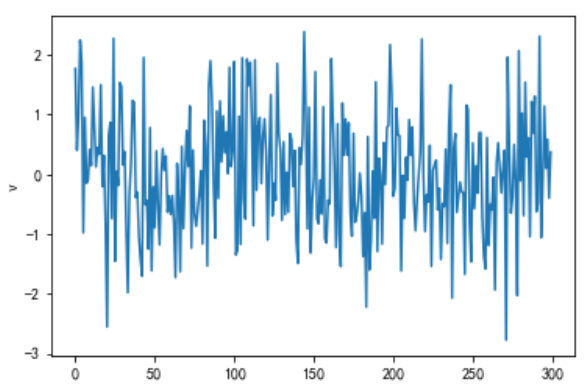
\includegraphics [width=0.6\textwidth]{fig/png_v.png}
	\caption{系统中添加的随机噪声}
	\label{fig:my_png_4}
\end{figure}


\section{总结}
BP神经网络是一种反向传播学习的非线性网络,以其具有自学习和自适应能力、泛化能力和优良的非线性映射能力,受到众多领域学者的关注。但是基于 BP 神经网络的系统辨识存在的网络初始权值的选择对辨识结果影响较大且不容易确定的缺点,改进 BP 算法有效地提高训练速度是我们下一步要研究的内容。
\newpage
\begin{appendices}
\section{程序代码}
\begin{lstlisting}[language=python,escapeinside=``]
import numpy as np
import matplotlib.pyplot as plt
%matplotlib inline
m1=1
m2=1
m3=1
m4=1
u=np.zeros((300),dtype=np.int)
for i in  range(300):
    u[i]=m1^m2
    m1=m2
    m2=m3
    m3=m4
    m4=u[i]
np.random.seed(0)
e = np.random.normal(0, 1, 300 )
z=np.zeros((300))
z[0]=0
z[1]=2
for i in range(2,300):
    z[i]=1.5*z[i-1]-0.7*z[i-2]+u[i-1]+0.5*u[i-2]+0.3*e[i]
x=[np.append(z[i-2:i],u[i-2:i]) for i in range(3,300)]
x=np.vstack(x)
y=z[3:].reshape((-1,1))
def tanh(x):
    return np.tanh(x)
def tanh_deriv(x):
    return 1.0 - np.tanh(x)*np.tanh(x)
def logistic(x):
    return 1/(1 + np.exp(-x))
class NeuralNetwork:
    def __init__(self, layers, activation='tanh'):
        if activation == 'logistic':
            self.activation = logistic
            self.activation_deriv = logistic
        elif activation == 'tanh':
            self.activation = tanh
            self.activation_deriv = tanh_deriv
        self.weights = []
        for i in range(1, len(layers) - 1):
            self.weights.append((2*np.random.random((layers[i - 1] , layers[i] ))-1)*0.25)
            self.weights.append((2*np.random.random((layers[i] , layers[i + 1]))-1)*0.25)
        self.errors=[]
    def fit(self, X, y, learning_rate=0.2, epochs=10000):
            X = np.atleast_2d(X)
            for k in range(epochs):
                i = np.random.randint(X.shape[0])
                a = [X[i]]
                for l in range(len(self.weights)):
                    a.append(self.activation(np.dot(a[l], self.weights[l])))
                self.error = y[i] - a[-1]
                self.errors.append(self.error[0])
                self.deltas = [self.error * self.activation_deriv(a[-1])]
                for l in range(len(a) - 2, 0, -1):
                    self.deltas.append(self.deltas[-1].dot(self.weights[l].T)
                    *self.activation_deriv(a[l]))
                self.deltas.reverse()
                for i in range(len(self.weights)):
                    layer = np.atleast_2d(a[i])
                    self.delta = np.atleast_2d(self.deltas[i])
                    self.weights[i] += learning_rate * layer.T.dot(self.delta)
    def predict(self, x):
            a = x
            for l in range(0, len(self.weights)):
                a = np.dot(a, self.weights[l])
            return a
nn=NeuralNetwork([4,10,10,1],'logistic')
nn.fit(x,y)
out=nn.predict(x)
\end{lstlisting}
\end{appendices}
	
\end{document}